\documentclass{beamer}
\usepackage{parskip}
\usepackage{tabularx}
\usepackage{booktabs}
\usetheme{Szeged}
\title{Contact timing in telemarketing campaigns}
\subtitle{Machine Learning for econometrics}
\author{Eléa Bordais, Jade Sillere, Eliott Von-Pine, Patryk Wiśniewski}
\date{Tuesday, April 1, 2025}

\begin{document}

\frame{\titlepage}

\begin{frame}
\frametitle{Table of contents}
\tableofcontents
\end{frame}

\section{Introduction}
\begin{frame}
\frametitle{Introduction}

\textbf{Objectives}: Identify the factors that influence a customer's likelihood of subscribing to term deposits during a marketing campaign. 

\textbf{Contribution}: Identify the impact of the time of the call on the likelihood of subscribing.


\textbf{Dataset}: Marketing dataset from a Portuguese banking institution of a marketing campaign from May 2008 to November 2010

\textbf{Methods}: Compare traditional causal inference methods with modern machine-learning based approaches

\vspace{0.5cm}

\end{frame}

\begin{frame}{Data overview}
\begin{figure}
    \centering
    \includegraphics[width=0.70\linewidth]{ressources/data_overview.png}
    \caption{Campaign process and observed data}
\end{figure}

\begin{itemize}
   \item Two types of contact : Inbound calls and outbound calls
   \item Most follow-up calls are at the request of the client
   \end{itemize}
\end{frame}

\begin{frame}{Overview of Variables}
\begin{itemize}
  \item \textbf{Outcome:} client subscribed to term deposit? (Yes or No)
  \item \textbf{Client variables:} age, job, marital status, education, loans, etc.
  \item \textbf{Contact variables: }communication type, month and day of last call, duration, number of contacts, info about previous campaign
  \item \textbf{State of the economy variables:} employment rate, consumer price index, consumer confidence index, 12-month euribor rate, etc.
\end{itemize}
\end{frame}


\section{Exploratory analysis}

\begin{frame}{Outcome and Campaign Organization}
\begin{figure}
    \centering
    \includegraphics[width=0.8\linewidth]{ressources/outcome.png}
\end{figure}
\begin{itemize}
    \item Outcome variable: Imbalance of "no" (88.7\%)
\end{itemize}

\end{frame}

\begin{frame}{Macroeconomic context}

\begin{figure}
    \centering
    \begin{minipage}[t]{0.55\linewidth}
        \centering
        \includegraphics[width=\linewidth]{ressources/euribor.png}
        \caption{Euribor 12mo rates}
    \end{minipage}%
    \hfill
    \begin{minipage}[t]{0.4\linewidth}
        \centering
        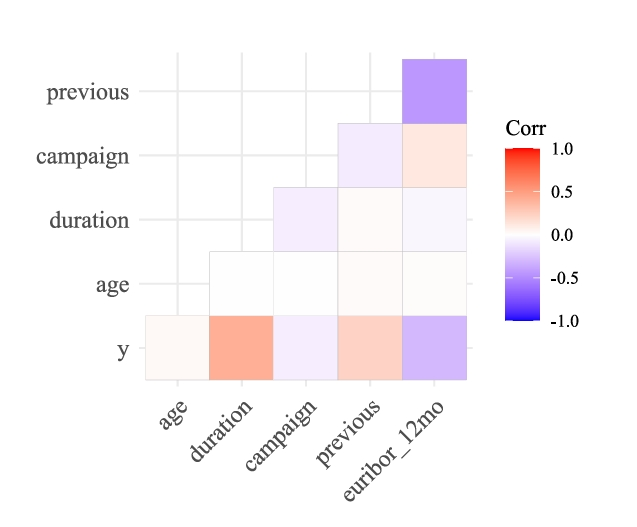
\includegraphics[width=\linewidth]{ressources/correlation.jpg}
        \caption{Correlation}
    \end{minipage}
\end{figure}
\vspace*{0.25cm}
A priori negative relation between interest rates and outcome, why?

\end{frame}


\begin{frame}{Time of Week: Naive approach}
\begin{table}[ht]
\centering
\begin{tabular}{lccccc}
\hline
\textbf{Share} & \textbf{Monday} & \textbf{Tuesday} & \textbf{Wednesday} & \textbf{Thursday} & \textbf{Friday} \\
\hline
Failure & 0.901 & 0.882 & 0.883 & 0.879 & 0.892 \\
Success & 0.099 & 0.118 & 0.117 & 0.121 & 0.108 \\
Count & 8514 & 8090 & 8134 & 8623 & 7823\\
\hline
\end{tabular}
\caption{Share of successful calls}
\end{table}
\begin{itemize}
    \item Calls close to uniformly distributed across days
    \item Higher success probabilities in the middle
\end{itemize}
\end{frame}


\section{Research question}
\begin{frame}{Timing of contact}
\begin{itemize}
    \item Hypotheses:
    \begin{itemize}
\item Calls in the middle of the week are more successful
\item Calls at the end of the month are more successful
\end{itemize}
     
    \item Idea:
    \begin{itemize}
        \item Leisure/Business mindset: in the middle of the week people are more rational, planning financials
        \item Catching-up/deadlines on Mondays/Fridays 
        \item Employees receive wage at the end month 
    \end{itemize}
\end{itemize}

\end{frame}

\begin{frame}{Timing of contact - PICO Formulation}
\small % Reduce text size
\renewcommand{\arraystretch}{1.2} 
\begin{tabular}{p{2cm} p{8cm}} 
\toprule
\textbf{Component} & \textbf{Description} \\
\midrule
\textbf{Population} & 
Customers from a Portuguese bank, contacted as part of a telemarketing campaign for a term deposit product \\
\textbf{Intervention} & 
Receiving a call during the middle of the week (Tue, Wed, Thur) / at the end of the month ($>$ 16th) \\
\textbf{Comparison} & Customers contacted another day \\
\textbf{Outcome} & Subscribing or not to the term deposit (probability) \\
\bottomrule
\end{tabular}
\end{frame}


\begin{frame}
\frametitle{Directed Acyclic Graph}
\begin{minipage}{0.51\linewidth}
\begin{figure}
    \centering
    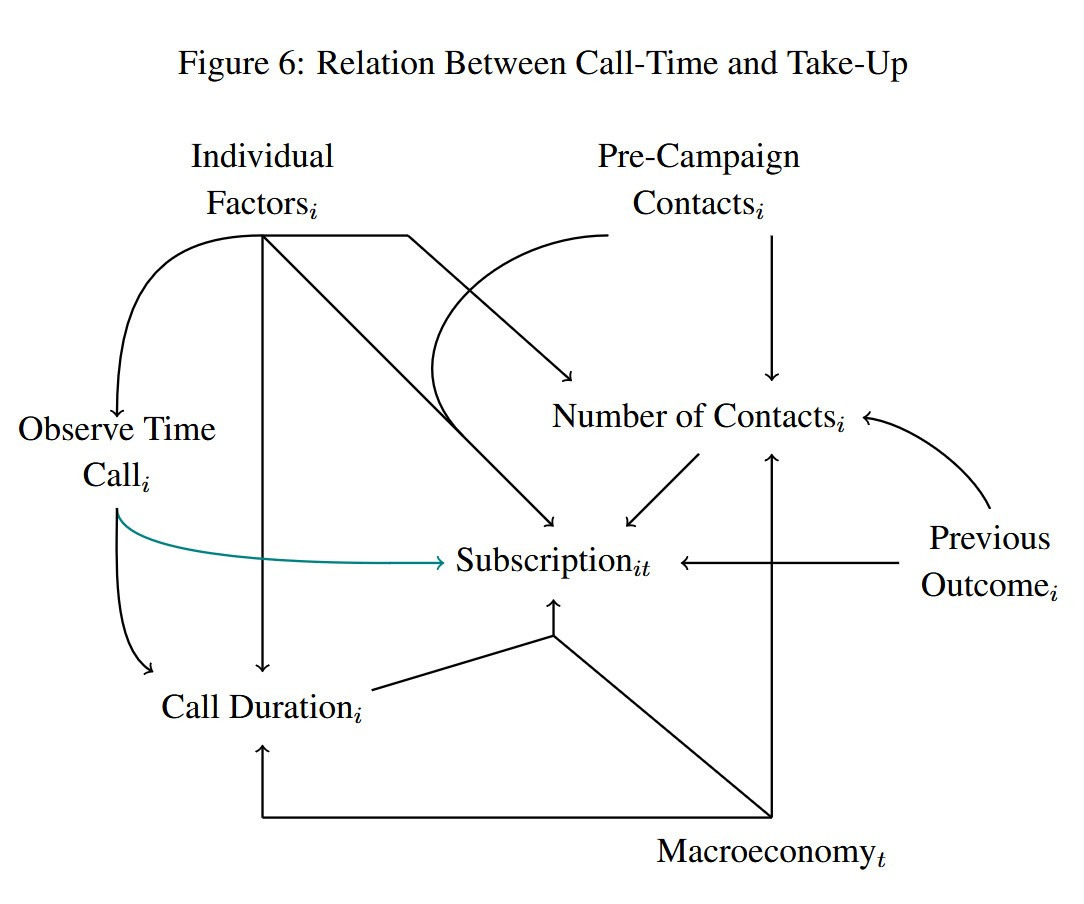
\includegraphics[width=1.05\linewidth]{ressources/dag.jpg}
\end{figure}
\end{minipage}
\hspace{0.4cm}
\begin{minipage}{0.43\linewidth}
\begin{itemize}
	\small
    \item  \textbf{Post-treatment:\\} $duration$
    \item \textbf{Unconfoundedness:\\} Bank calls uniformly across days 
    \item \textbf{Overlap:} Treated and control have comparable characteristics
\end{itemize}
\end{minipage} 
\end{frame}

\section{Methodology}

\begin{frame}{Data pre-processing and imputation}
\begin{itemize}
    \item Recoded missing values
    \item Filtered for clients only contacted a single time during the campaign
    \item Converted the numeric pdays value to 3 categories (never contacted, contacted within a week and contacted beyond a week)
    \item Imputation using the MICE approach
\end{itemize}
\end{frame}

\begin{frame}{Imputation Method: \texttt{mice} Package}
Assuming missing values are MAR (Missing At Random), I used the \texttt{mice} package with default imputation functions to generate 5 imputed datasets:
\begin{itemize}
	\small
    \item \texttt{pmm}: Predictive Mean Matching (numeric data)
    \item \texttt{logreg}: Logistic Regression (binary data, 2 levels)
    \item \texttt{polyreg}: Polytomous Regression (unordered categorical, $>2$ levels)
    \item \texttt{polr}: Proportional Odds Model (ordered categorical, $>2$ levels)
\end{itemize}

The number of imputations is supported by literature (Bennet, 2001; Hawthorne and Eliott, 2005 and Royston et al.).
\end{frame}

\begin{frame}{Estimators}

\begin{itemize}
    \item Simple Logit
    \item Double Machine Learning - PLM and IRM
    \begin{itemize}
        \item Random forest + tuning hyperparameters
        \item Ensemble (for PLM only) using the following estimators for the classifiers/regressors:
        \begin{itemize}
            \item Random Forest, Logit (classifier only), Neural Net, linear model (regressor only), XGBoost (regressor only)
        \end{itemize}
    \end{itemize}
    \item Causal Random Forest
\end{itemize}

\end{frame}

\section{Results}

\begin{frame}{Moment of the week}
\begin{figure}[h!]
    \centering
    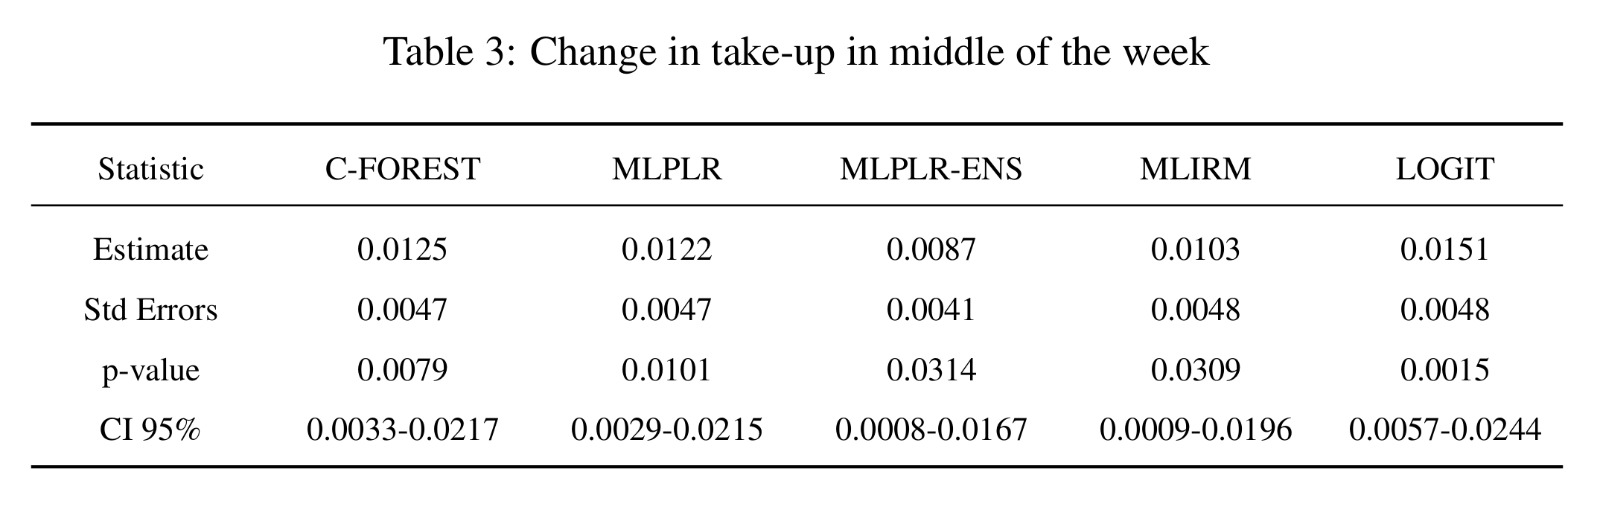
\includegraphics[width=1\textwidth]{ressources/tbl3.jpg}
\end{figure}

\begin{itemize}
\item Statistically significant results in all models
\item Largest coefficient with logit, smallest with PLR-ENS
\end{itemize}

\end{frame}

\begin{frame}{Moment of the Month}
\begin{figure}[h!]
    \centering
    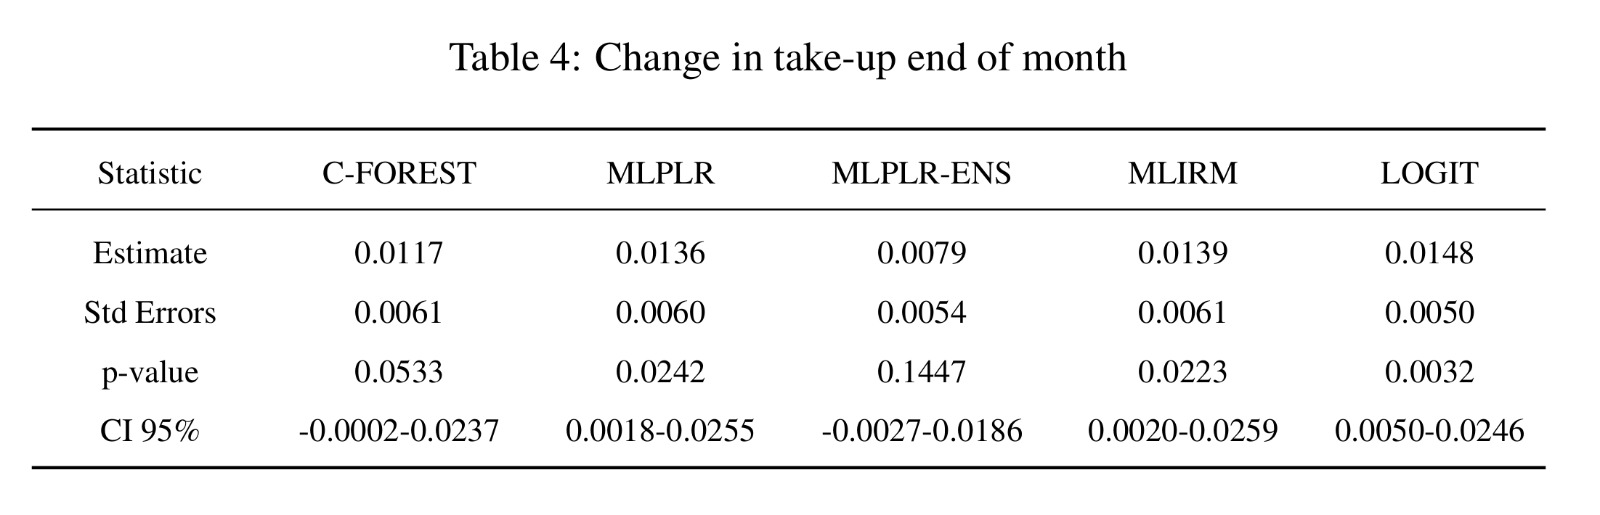
\includegraphics[width=1\textwidth]{ressources/tbl4.jpg}
\end{figure}
\begin{itemize}
\item Coefficients not always significant
\item Again, largest coefficient with logit, smallest with PLR-ENS
\end{itemize}
\end{frame}

\begin{frame}{Moment of the Week (Heterogeneity)}
\begin{figure}[h!]
    \centering
    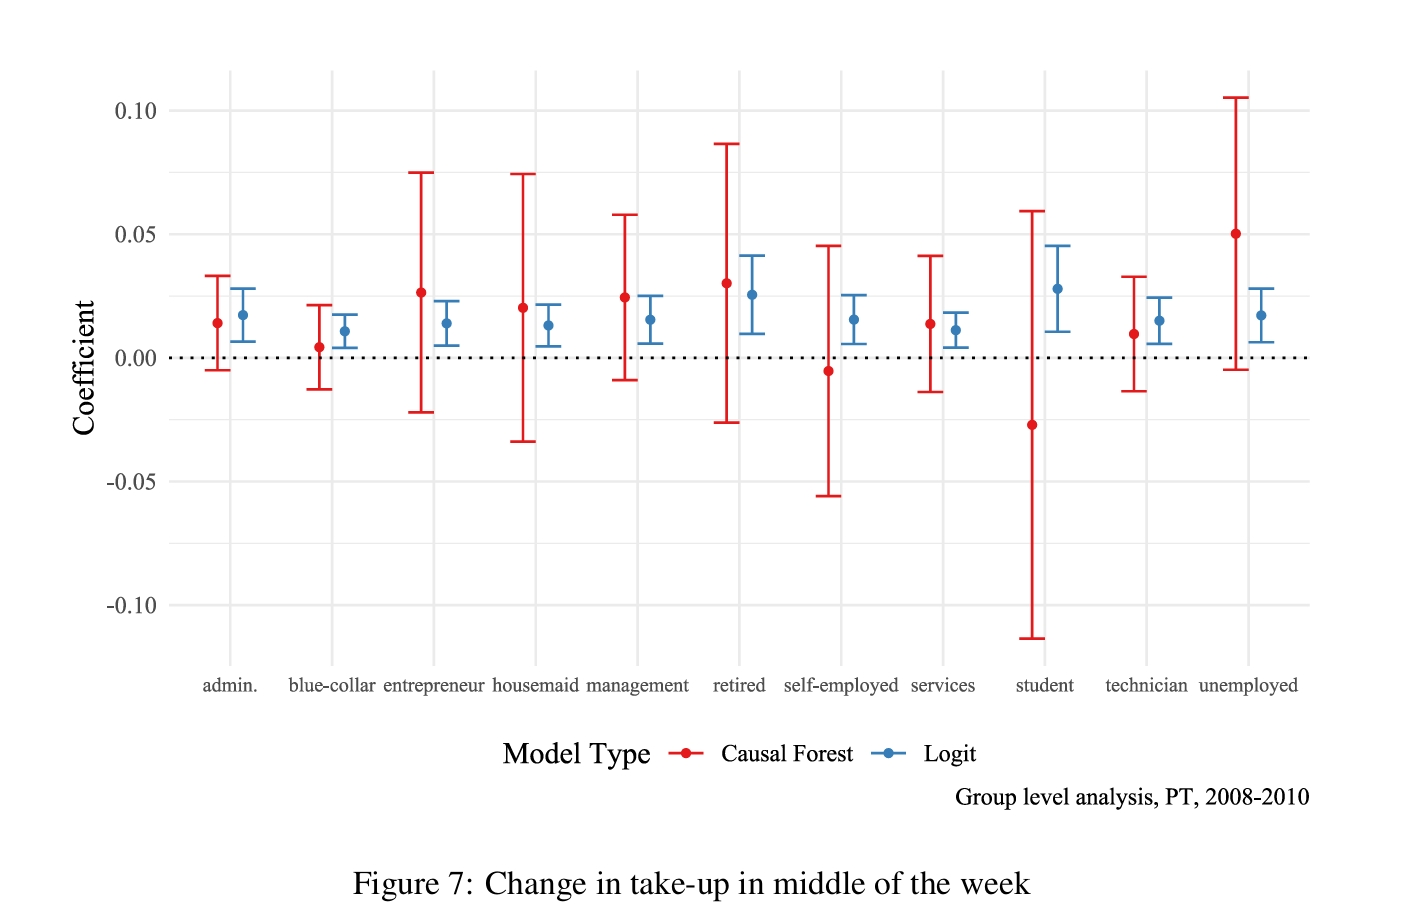
\includegraphics[width=.9\textwidth]{ressources/fig7.jpeg}
\end{figure}
\end{frame}

\begin{frame}{Moment of the Month (Heterogeneity)}
\begin{figure}[h!]
    \centering
    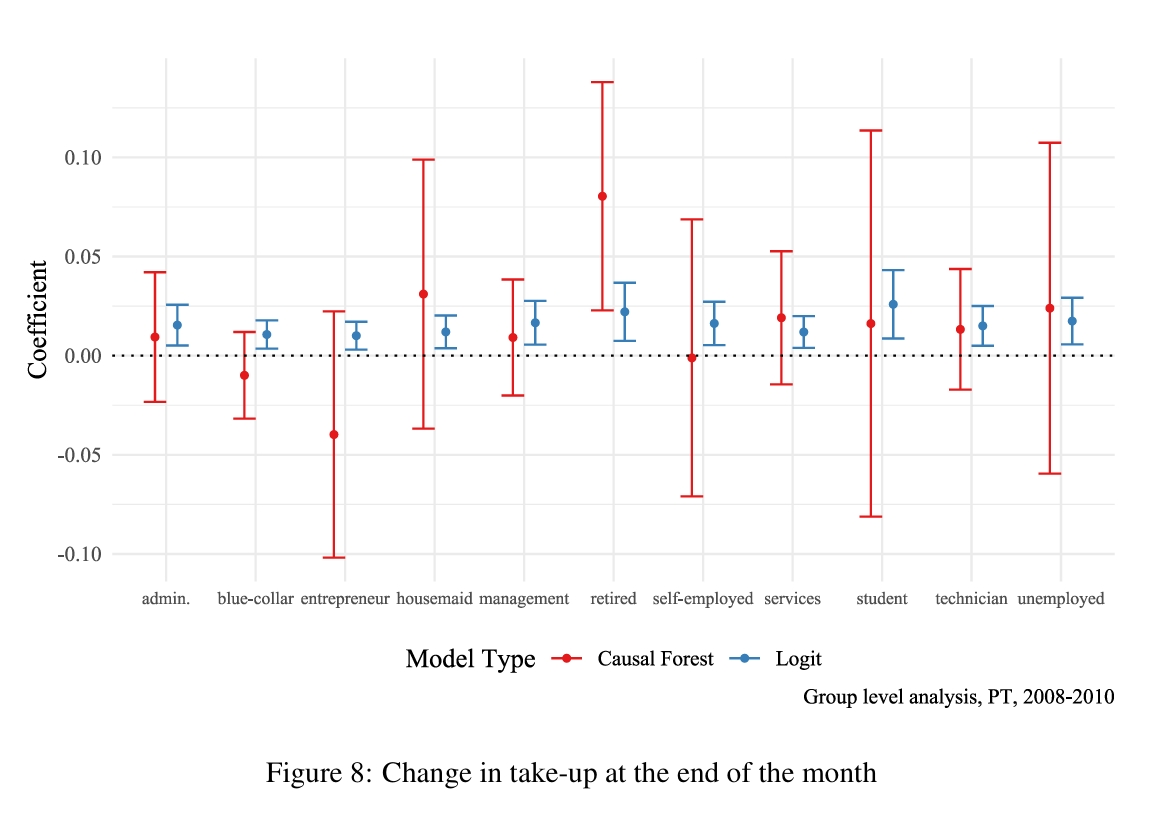
\includegraphics[width=.9\textwidth]{ressources/fig8.jpeg}
\end{figure}
\end{frame}

\section{Interest Rates}
\begin{frame}{DAG, PICO and Macro}
\begin{figure}[h!]
    \centering
    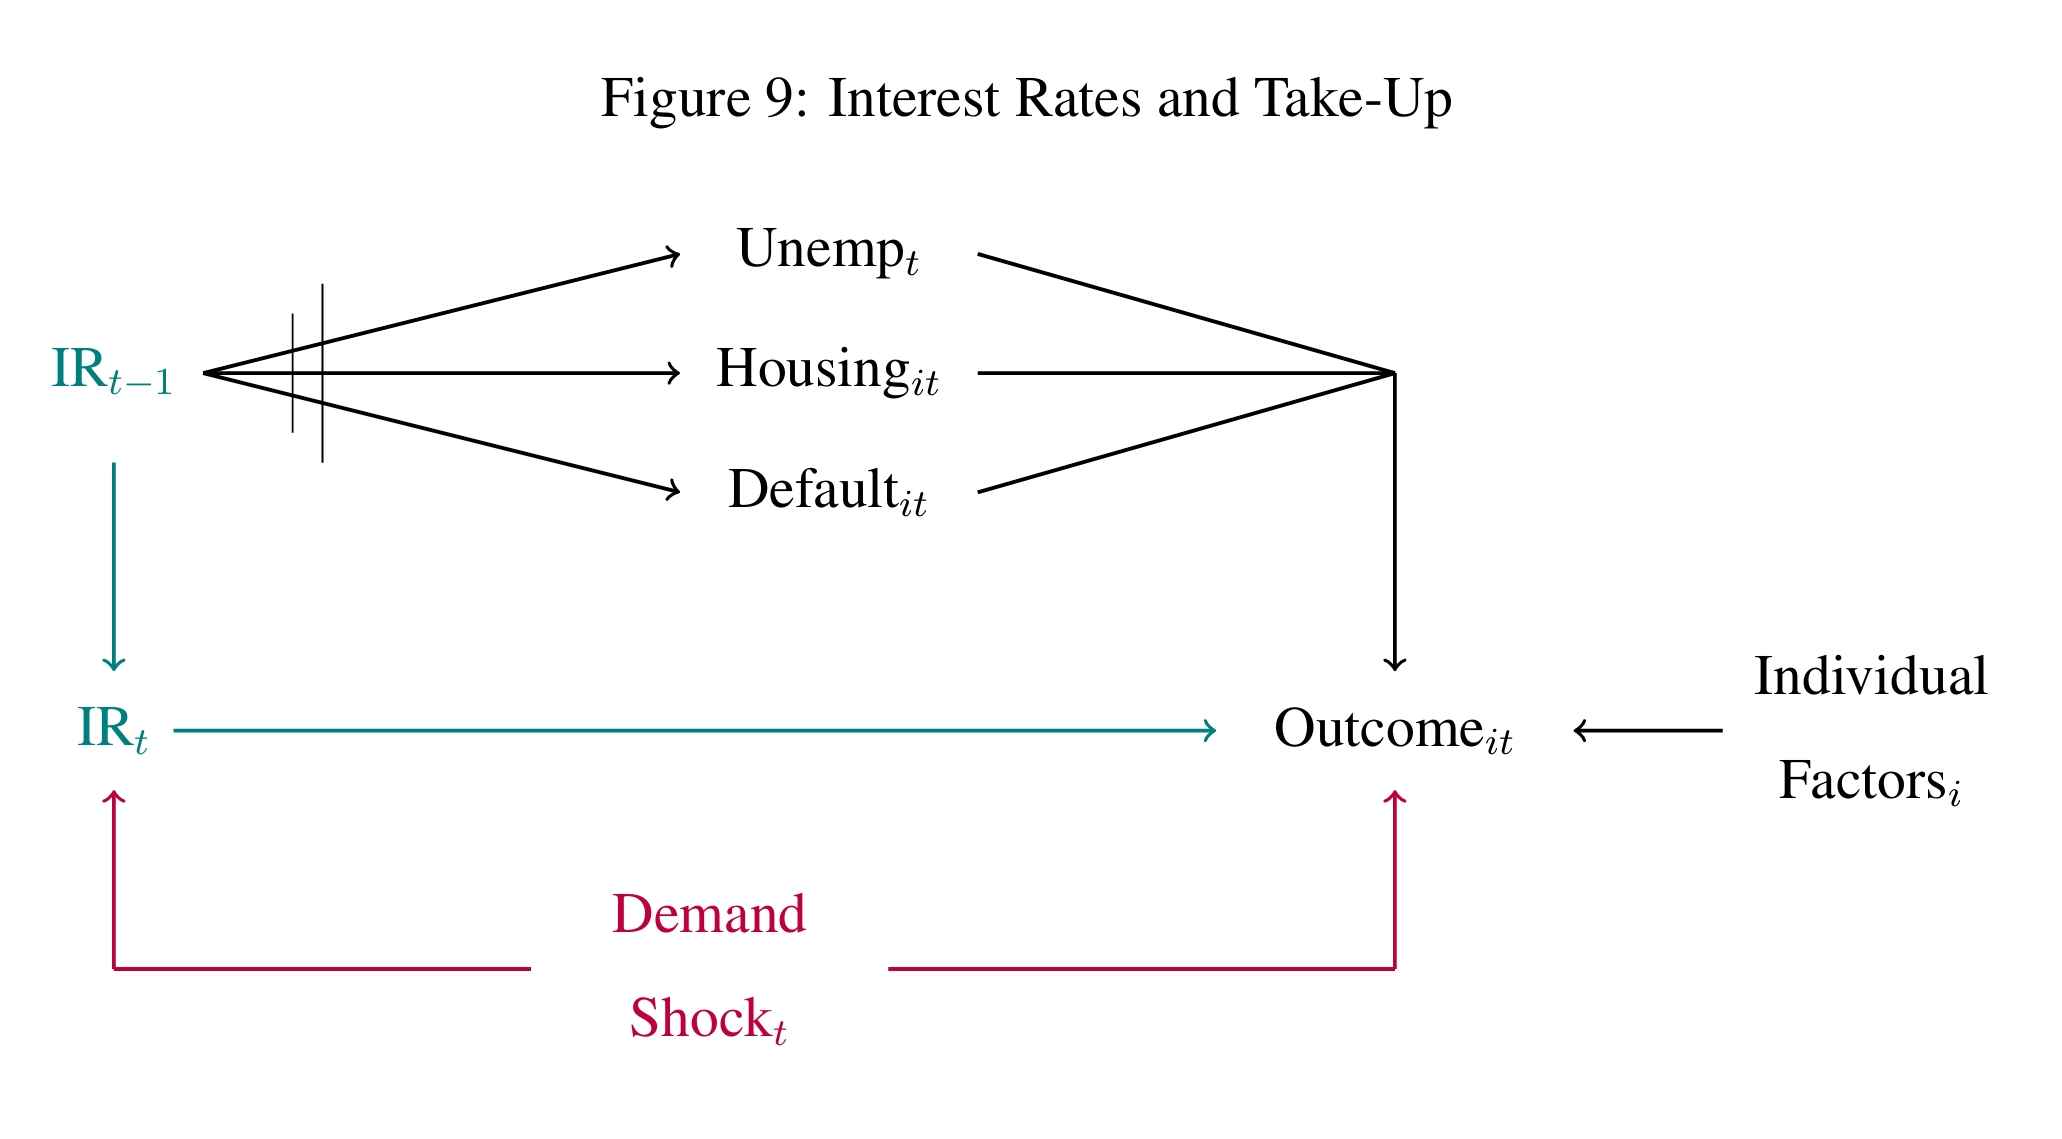
\includegraphics[width=.88\textwidth]{ressources/fig9.jpeg}
\end{figure}
\vspace*{-0.25cm}
Interest rates are prices, so they relate both to demand and supply.

\end{frame}

\begin{frame}{Interest Rate Effects}
\begin{figure}[h!]
    \centering
    \includegraphics[width=.9\textwidth]{ressources/tbl5.PNG}
\end{figure}

- LPM likely over-estimating the effects

- DML-IV less rigid than Probit-IV

\end{frame}

\section{Conclusion}
\begin{frame}{Conclusion}

Take home message:
\begin{itemize}
\item Timing in marketing matters not only \emph{who?} but \emph{when?}
\item Careful about endogeneity when working with prices
\end{itemize}

Some of the limits of what we've shown:
\begin{itemize}
\item Individuals that do not pickup are not observed
\item Simulation exercise needed to better compare methods
\item External validity not guaranteed 
\item Instrument validity 
\end{itemize}


\end{frame}

\end{document}